
\section{Grundlagen}
\label{sec:Grundlagen}
\subsection{Einleitung}

\subsection{Genetische Algorithmen}

\subsection{Aufbau eines GA in Einzelschritten}
\subsubsection{Initzialisierung der Population}
\subsubsection{Grade}
\subsubsection{Evolve}
\paragraph{Select Parents}
\paragraph{Breed}
\paragraph{Exchange}
\subsubsection{Loop}

\newpage

\subsection{Künstliche Neuronale Netze}


\begin{figure}[htb]
  \centering  
  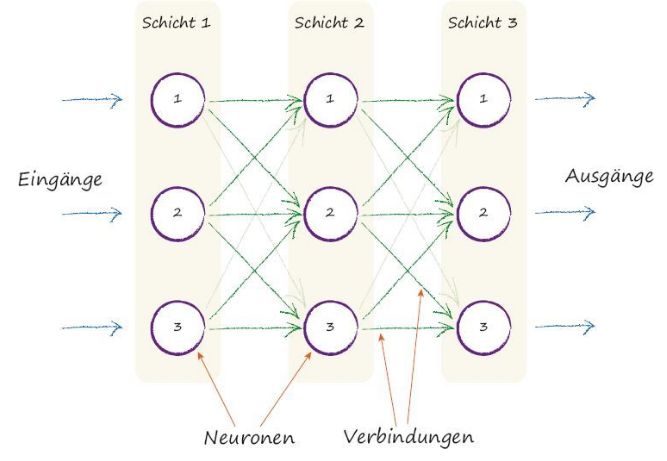
\includegraphics[scale=0.5]{img/S36_Buildyourown.png}
  \caption{Neuronales Netz   \cite{rashid2017neuronale}}
  \label{fig:neural_network}
\end{figure}


Hier zu sehen ist ein Künstliches Neuronales Netz mit drei Schichten \ref{fig:neural_network}. Dies wurde dem natürlichen Vorbild der neuronalen Netze im Gehirn nach empfunden. Die Kreise nennt man Neuronen, mehrere Neuronen zusammen ergeben eine Schicht oder auch Layer genannt. Die Verbindungen repräsentieren die Gewichte, über diese kann einem Netz verschiedene Zusammenhänge von Input und Output antrainiert bzw. angelernt werden. Zum Training werden viele Daten benötigt, aus welchen das Netz \glqq Lernt\grqq{}. Dafür ist es wichtig, viele aufbereitete Daten zu besitzen, denn diese Netze brauchen viele Trainingsiterationen, bis das gewünschte Ergebnis zustande kommt. Ein Neuron besteht aus Eingängen, Gewichten und einer Aktivierungfunktion sowie einem Ausgang. Die Vernetzung mehrerer Neuronenschichten lässt ein Neuronales Netz entstehen.

\newpage



\subsection{Aufbau eines Neurons}
\begin{figure}[htb]
  \centering  
  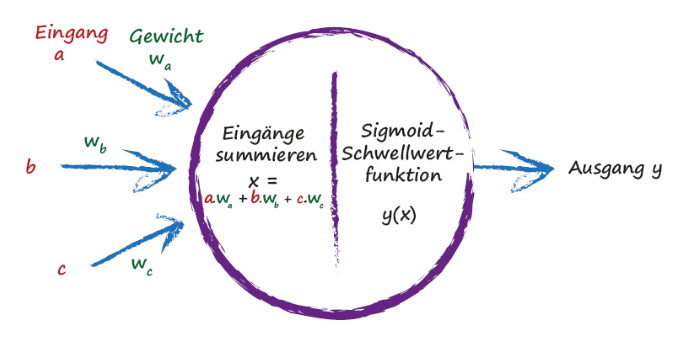
\includegraphics[scale=0.5]{img/S41_Buildyourown.png}
  \caption{Aufbau eines Neurons  \cite{rashid2017neuronale}}
  \label{fig:neuron}

\end{figure}
\subsubsection{Eingang aka Input}
Bei dem Input handelt es sich um einfache xxxFloatwer dieser wird mit den einzelnen Gewichten verrechnet. Ein Neuron hat meist mehrere Eingangsgrößen welche alle zusammen mit den gewichten aufsummiert werden. Diese Werte werden zufällig initialisiert und per Training verbessert, somit handelt es sich um einen angelernten Werte, welche durch die Backproagation (Fehlerrückführung) verbessert werden.

\subsubsection{Offset aka bias}
Auf dieses Aufsummiertes Ergebniss wird anschließend ein Bias gerechnet, dieser führt zu einem besseren Verhalten beim Trainieren. Bei diesen Werten handelt es sich um angelernte Werte, die per Backpropagation verbessert werden und die Flexibitlität der Netze erhöht.


\subsubsection{Aktivierungs Funktion}
Die Aktivierungsfunktion kann man sich als Schwellwert vorstellen, ab wann das Neuron den Input weiter gibt. Es gibt verschiedene Funktionen, um diesen Schwellwert zu definieren. Je nach Aufgabe des Neuronalen Netze werden andere Aktivierungsfunktionen verwendet. Bei Klassifizierungen werden heute meist ReLu-Layer oder ein Weakly-ReLu Layer benutzt, diese verhindern das Vanishing- bzw. Exploding- gradientproblem beim Trainieren.

\subsubsection{Ausgang aka Output}
Wenn der Schwellwert überschritten wird, wird am Output durchgeschaltet. Dieser Output kann entweder mit einer nen Schicht Neronen verbundne sein oder direkt als Ausgang gesehen werden. Über welchen man anhand von xxxVariabelenwerten/Kommawerten die 
Von Input nach Output nennt sich ein Single-Forward-Pass. Wie hier beschrieben wird, kann ein Netz verschieden viele Layer besitzen mit verschiedenen Anzahlen von Neuronen.

\subsection{Verlustfunktion aka lossfunktion}
Die Verlustfunktion stellt ein ausgesuchtes Maß der Diskrepanz zwischen den beobachteten und den vorhergesagten Daten dar. Sie bestimmt die Leistungsfähigkeit des neuronalen Netzes während des Trainings und der Ausführung. Ziel ist es, im laufenden Prozess der Modellanpassung, die Verlustfunktion zu minimieren.

\subsection{Optimierer alt Gradientenabstieg}
Um die Fehlerfunktion zu minimieren wird als Werkzeug der Gradienten Abstieg benutzt. Diese ist nur möglich da ein Künstliches Neuronales Netz aus verketteten differenzierbaren Gewichte der Neuronen(Tensoroperationen) aufgebaut ist, die es erlauben duch anwendung der Kettenregel die Gradientenfunktion zu finden, die den aktuellen Parametern des Datenstapels werte des Gradienten zuordnet. Es gibt auch hier verschiedene Ansätze von Optimierern, welche die genauen Regeln wie der Gradient der Verlustfunktion zu Aktualisierund der Parameter verwendet wird hier könnte Beispielweise den RMSProp-Optimierer, der die trägheit des Gradientenabstiegsverfahren berücksichtet. Seite 83 - Deep Learning chollet


\iffalse
 Im Grunde werden dabei die Gewichte so angepasst, dass ein besseres Ergebnis entsteht und dadurch die Fehlerfunktion verringert wird. Wie das Wort Backpropagation schon sagt, wird von hinten nach vorne verbessert. Es gibt verschiedene Variationen von Gradientenabstiegen, welche verschiedene Vor- und Nachteile haben. Bei dem Trainieren des Netzes wurde der Momentum-Optimizer, welcher aus einem Gradientenabstieg mit Momentum aufgebaut ist.
\fi


\subsection{Lern Methoden des Maschine Learnings}
Es gibt vier verschiedene Lernmethoden beim Maschinellen Lernens, überwachtes, unüberwachtes, selbstüberwachtes und verstärkendes Lernen. Es werden aus Zeitgründen nur die wichtigsten zwei Besprochen.

\subsubsection{Überwachtetes Lernen aka Supervised Learning}
Überwachtes Lernen wird dafür benutzt, eine Funktion zu finden, Daten einem Wert zuzuweisen. Dennoch müssen dafür alle Daten meist von einem Menschen vorverarbeitet werden und eine Beschriftung/Zielwert(eng. Label) zugeordnet werden. Damit das Netz auch eine Aussage über das Ergebnis, während des Trainings, geben kann. Anwendungsfälle sind Regression, Klassifikation und Empfehlungen.

\subsubsection{Unüberwachtes Lernen aka Unsupervised Learning}
Im Vergleich zum überwachten Lernen liegen hier keine Zielinformationen (eng. Labelinformation) vor. Weshalb dieser Ansatz eher zum Erkennen von Mustern und Ableiten von Regeln da ist. Für unsupervised Leaning Algorithem sind in der Regel sehr viele Daten nötig. Anwendungsgebiete für Unüberwachtes lernen sind das Clustering und die Dimensionsreduktion.

\subsection{Hyperparameter}
Als Hyperparameter werden, in Bezug auf KNN's, meist die Anfangsbedingungen bezeichnet. Im Klassischenfall wären dies die Learnrate (eng. Learningrate), der Abdeckunggrad(eng. Dropout), die verlustfunktion oder auch der Optimizer. In selten fällen kann man die Modelachitektur auch als Hyperparameter bezeichen. Für diese Hyperparameter gelten keine universellen Werte sondern müssen je nach Daten und Funktion (oder KNN)speziell angepasst und verändert werden. Deshalb gibt es nur einige Regeln und grobe abschätzungen wie diese Hyperparameter aussehen sollen. 

\subsection{Zusammenfassung}